\section{Vom Induktionsbeweis zum rekursiven Algorithmus}

\begin{example}[Türme von Hanoi]~
\begin{center}
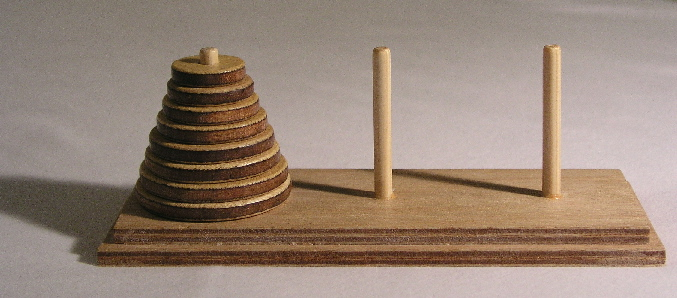
\includegraphics[width=0.8\textwidth]{figures/hanoi}
\end{center}
\begin{quote}
``Die Türme von Hanoi''\footnote{Beschreibung und Bild von Wikipedia.} ist ein Geduldspiel. Das Spiel besteht aus drei gleich grossen Stäben A, B und C, auf die mehrere gelochte Scheiben gelegt werden, alle verschieden gross. Zu Beginn liegen alle Scheiben auf Stab A, der Grösse nach geordnet, mit der grössten Scheibe unten und der kleinsten oben. Ziel des Spiels ist es, den kompletten Scheiben-Stapel von A nach C zu versetzen.
Bei jedem Zug darf die oberste Scheibe eines beliebigen Stabes auf einen der beiden anderen Stäbe gelegt werden, vorausgesetzt, dort liegt nicht schon eine kleinere Scheibe. Folglich sind zu jedem Zeitpunkt des Spieles die Scheiben auf jedem Feld der Grösse nach geordnet.
\end{quote}
Wir wollen beweisen, dass ``die Türme von Hanoi'' mit beliebig vielen Scheiben erfolgreich gespielt werden können.
\begin{proof} Wir benutzen ein Induktionsargument ($n$ sei die Anzahl Scheiben):
\begin{itemize}
\item \textbf{Verankerung $n=0$:} Dieser Fall ist trivial, da es keine Scheiben zu bewegen gibt.
\item \textbf{Induktionsschritt $n\to n+1$:} Wir betrachten das Spiel mit $n+1$ Scheiben. Nach Induktionsvoraussetzung gibt es eine Lösungsstrategie für das Spiel mit nur $n$ Scheiben. Diese Strategie können wir offensichtlich dazu verwenden, um alle bis auf die grösste Scheibe auf den Stab B zu verschieben. Nun können wir die grösste Scheibe auf den Stab $C$ verschieben, um anschliessend nochmal die Strategie für das Spiel mit $n$ Scheiben anzuwenden und alle kleineren Scheiben auf den Stab C zu bewegen. Das Spiel ist somit auch für $n+1$ Scheiben lösbar. \qedhere
\end{itemize}
\end{proof}
\begin{remark}
Der Beweis, dass die Türme von Hanoi für beliebige $n$ gelöst werden können, ist mehr als nur eine Argumentationskette, die dazu geeignet ist jemanden davon zu überzeugen, dass es tatsächlich \textit{irgendwie möglich sein muss} das Spiel zu gewinnen. Es steckt viel mehr in diesem Beweis; der Beweis gibt einen konkreten Algorithmus (rekursiv) vor, wie das Spiel erfolgreich gespielt werden kann. Wir betrachten eine Implementierung dieser Lösungsstrategie in Java.


\lstset{language=Java}
\begin{framed}
\begin{lstlisting}
// x-viele Scheiben von A nach B verschieben:
// Falls x=0, dann ist nichts zu tun.
// Sonst, zuerst die oberen (x-1) Scheiben von A nach C
// verschieben,
// dann die groesste Scheibe von A nach B verschieben
// und schliesslich alle anderen Scheiben von C nach B
// verschieben
public class HanoiSolver{

    public String solve(int size){
        return AC(size);
    }

    private String AB(int x){
        if (x==0) return "";
        return AC(x-1)+" AB "+CB(x-1);
    }

    private String AC(int x){
            if (x==0) return "";
            return AB(x-1)+" AC "+BC(x-1);
    }

    private String BC(int x){
            if (x==0) return "";
            return BA(x-1)+" BC "+AC(x-1);
    }

    private String BA(int x){
            if (x==0) return "";
            return BC(x-1)+" BA "+CA(x-1);
    }

    private String CB(int x){
            if (x==0) return "";
            return CA(x-1)+" CB "+AB(x-1);
    }

    private String CA(int x){
            if (x==0) return "";
            return CB(x-1)+" CA "+BA(x-1);
    }
}
\end{lstlisting}
\end{framed}
und die kurze Fassung:
\begin{framed}
\begin{lstlisting}
public class HanoiSolverCompact{

    public String solve(int size){
        return hanoi("A","C","B",size);
    }

    private String hanoi(String x,String y,String z,int n){
        if(n==0) return "";
        return hanoi(x,z,y,n-1)+" "+x+y+hanoi(z,y,x,n-1);
    }
}
\end{lstlisting}
\end{framed}

%\begin{lstlisting}
%let rec AB x =
%    if x=0 then []
%    else (CB (x-1))@(('A','B')::(AC (x-1)))
%
%and AC x =
%    if x=0 then []
%    else (BC (x-1))@(('A','C')::(AB (x-1)))
%
%and BC x =
%    if x=0 then []
%    else (AC (x-1))@(('B','C')::(BA (x-1)))
%
%and BA x =
%    if x=0 then []
%    else (CA (x-1))@(('B','A')::(BC (x-1)))
%
%and CB x =
%    if x=0 then []
%    else (AB (x-1))@(('C','B')::(CA (x-1)))
%
%and CA x =
%    if x=0 then []
%    else (BA (x-1))@(('C','A')::(CB (x-1)))
%
%\end{lstlisting}
\end{remark}
\end{example}


\begin{example}\label{bsp:plättli}
Ist es immer möglich ein ``gelochtes $n\times n$-Quadrat''
\begin{center}
\begin{tabular}{ | c | c | c | c | c  | c | c | c | }
\hline
&&&&&&&\\
\hline
&&&&&&&\\
\hline
&&&&&&&\\
\hline
&&&&&&&\\
\hline
&&&&&&\cellcolor{black}&\\
\hline
&&&&&&&\\
\hline
&&&&&&&\\
\hline
&&&&&&&\\
\hline
\end{tabular}
\end{center}

mit Flächen von der Form
\begin{tabular}{ c c }
&\cellcolor{black}\\
\cellcolor{black}&\cellcolor{black}
\end{tabular}
``passgenau'' zu überdecken? Ja, wenn $n$ eine Zweierpotenz ist. Wir können diese Behauptung durch Induktion wie folgt beweisen:  Wir nehmen an, dass das ``gelochte Quadrat'' eine Seitenlänge von $2^n$ hat.
\begin{itemize}
\item Verankerung ($n=0$): Wenn $n=0$, dann besteht das gelochte Quadrat nur aus einem Loch. Wir können das Quadrat (ohne etwas zu tun) überdecken.
\item Hat das Quadrat die Seitenlänge $2^{n+1}$, dann zerlegen wir es in vier gleich grosse Quadranten, die alle die Seitenlänge $2^n$ haben. Wir platzieren eine der Flächen wie unten angedeutet (rot).
\begin{center}
\begin{tabular}{ | c | c | c | c !{\color{red}\vrule} c  | c | c | c | }
\hline
&&&&&&&\\
\hline
&&&&&&&\\
\hline
&&&&&&&\\
\hline
&&&\cellcolor{red}&\cellcolor{red}&&&\\
\arrayrulecolor{red}\hline
\arrayrulecolor{black}&&&\cellcolor{red}&&&&\\
\hline
&&&&&&\cellcolor{black}&\\
\hline
&&&&&&&\\
\hline
&&&&&&&\\
\hline
\end{tabular}
\end{center}
Nun sind alle Quadranten ein ``gelochtes Quadrat'' der Seitenlänge $2^n$. Wir können also nach Induktionsvoraussetzung alle Quadranten passgenau belegen.
\end{itemize}
\end{example}

\begin{example}
Implementieren Sie (ausgehend vom Beispiel~\ref{bsp:plättli}) in einer Programmiersprache Ihrer Wahl, einen Algorithmus zur Überdeckung von ``gelochten Quadraten'', die eine Zweierpotenz als Seitenlänge haben.
\end{example}